\documentclass{beamer}
\usepackage{wasysym}

\usepackage[framemethod=tikz]{mdframed}
\usepackage[makeroom]{cancel}
\usepackage{tikz}

\tikzstyle{every picture}+=[remember picture]
\usetikzlibrary{arrows,positioning}
\tikzset{
	%Define standard arrow tip
	>=stealth',
	%Define style for boxes
	punkt/.style={
		rectangle,
		rounded corners,
		draw=black, very thick,
		text width=6.5em,
		minimum height=2em,
		text centered},
	% Define arrow style
	pil/.style={
		->,
		thick,
		shorten <=2pt,
		shorten >=2pt,}
}
\usetikzlibrary{positioning}

\usetheme[sectionpage=none,numbering=counter]{metropolis}
%\setbeamertemplate{footline}[frame number]
\usepackage{graphicx}
\usepackage[utf8]{inputenc}
\usepackage[T1]{fontenc} 
\newcommand{\textoverscript}[1]{$^{\text{#1}}$}
\newcommand{\textunderscript}[1]{$_{\text{#1}}$}
\usepackage{caption}
\captionsetup{justification=raggedright,singlelinecheck=false}
\captionsetup[figure]{labelformat=empty}


\setbeamercovered{transparent}% Dim out "inactive" elements
\setbeamertemplate{caption}{\raggedright\insertcaption\par}
\setlength\abovecaptionskip{-15pt}
\newcommand{\tabitem}{%
  \usebeamertemplate{itemize item}\hspace*{\labelsep}}
\title{He$^+$ Pickup Ion Measurements\\ with Ulysses SWICS}
\subtitle{MNF-phys-1321}
%\subtitle{MNF-phys-1321 -- Methodenkenntnisse und Projektplanung}
\author{Anne Fischer}
\date{\today}
%
%
%
\begin{document}

%%%
\begin{frame}{Pickup Ion measurements with SWICS (Ulysses)}

	\begin{figure}
		\vspace{.3cm}
		\includegraphics[scale=0.25]{Pics/PU_process.pdf}
		\vspace{0.8cm}
	\end{figure}
\end{frame}
% ***********
\begin{frame}

\begin{center}
	{\footnotesize \textbf{SWICS}: \textbf{S}olar \textbf{W}ind \textbf{I}on \textbf{C}omposition\textbf{ S}pectrometer \\ \vspace{-0.1cm} -- a Time-of-flight mass spectrometer}
\end{center}
\begin{columns}
	\column{0.4\textwidth}
	\begin{figure}		
		\vspace{-.55cm}	
		\includegraphics[scale=0.2]{Pics/ulysses_trajectory.pdf}
	\end{figure}
	\begin{figure}
		\vspace{.3cm}
		\includegraphics[scale=0.05]{Pics/ULYSSES-SWICS.jpg}
		\vspace{0.8cm}
	\end{figure}


\column{0.55\textwidth}
			\begin{figure}		
		\vspace{-.8cm}
		\includegraphics[scale=0.14]{Pics/SWICS_measurement_gerade.pdf}
		\caption{\tiny{\begin{center}
					\textit{Gloeckler, Geiss et al., 1992}\end{center}}}
		
	\end{figure}
		
		\vspace{-.4cm}
		\begin{itemize}
			\begin{footnotesize}		
				\item $\left\{\frac{E}{q}, ToF, E_{SSD}\right\}$ $\Rightarrow \left\{\frac{M}{q}, M, |v|\right\}$ 
				\item identification \& energy of the ion 
			\end{footnotesize}
		\end{itemize}
\end{columns}
\vspace{0.5cm}
\end{frame}
% ***********
\begin{frame}
\begin{center}
	\textbf{Velocity Distributions: 1D vs. 3D}
\end{center}

\begin{columns}
	\column{0.5\textwidth}
	\begin{figure}
		\vspace{-1.2cm}			
		\includegraphics[scale=0.18]{Pics/qm.pdf}
		\caption{\tiny{\begin{center}
					\textit{Gloeckler, Geiss et al., 1992}\end{center}}}
	\end{figure}
	
	{\footnotesize \begin{itemize}
			\item Sectorization of the SWICS sensor
			\item Rotation of SWICS
			\item Aspect Angle
	\end{itemize}}
	
	\column{0.5\textwidth}
	\begin{figure}		
		%\vspace{1.1cm}	
		\includegraphics[scale=0.26]{Pics/cart_50_counts_R.pdf}
	\end{figure}
	
	\begin{figure}		
		\vspace{-0.5cm}	
		\includegraphics[scale=0.1]{Pics/swics_sensor_flipped_rotated_arrows.pdf}
	\end{figure}
\end{columns}
\end{frame}


%%%%
%\begin{frame}{}
%\vspace{-0.5cm}
%\begin{columns}				
%\column{5cm}
%\begin{figure}				
%	\includegraphics[scale=0.13]{Pics/swics_sensor_flipped_rotated_arrows.pdf}
%\end{figure}
%\column{5cm}
%\begin{figure}				
%	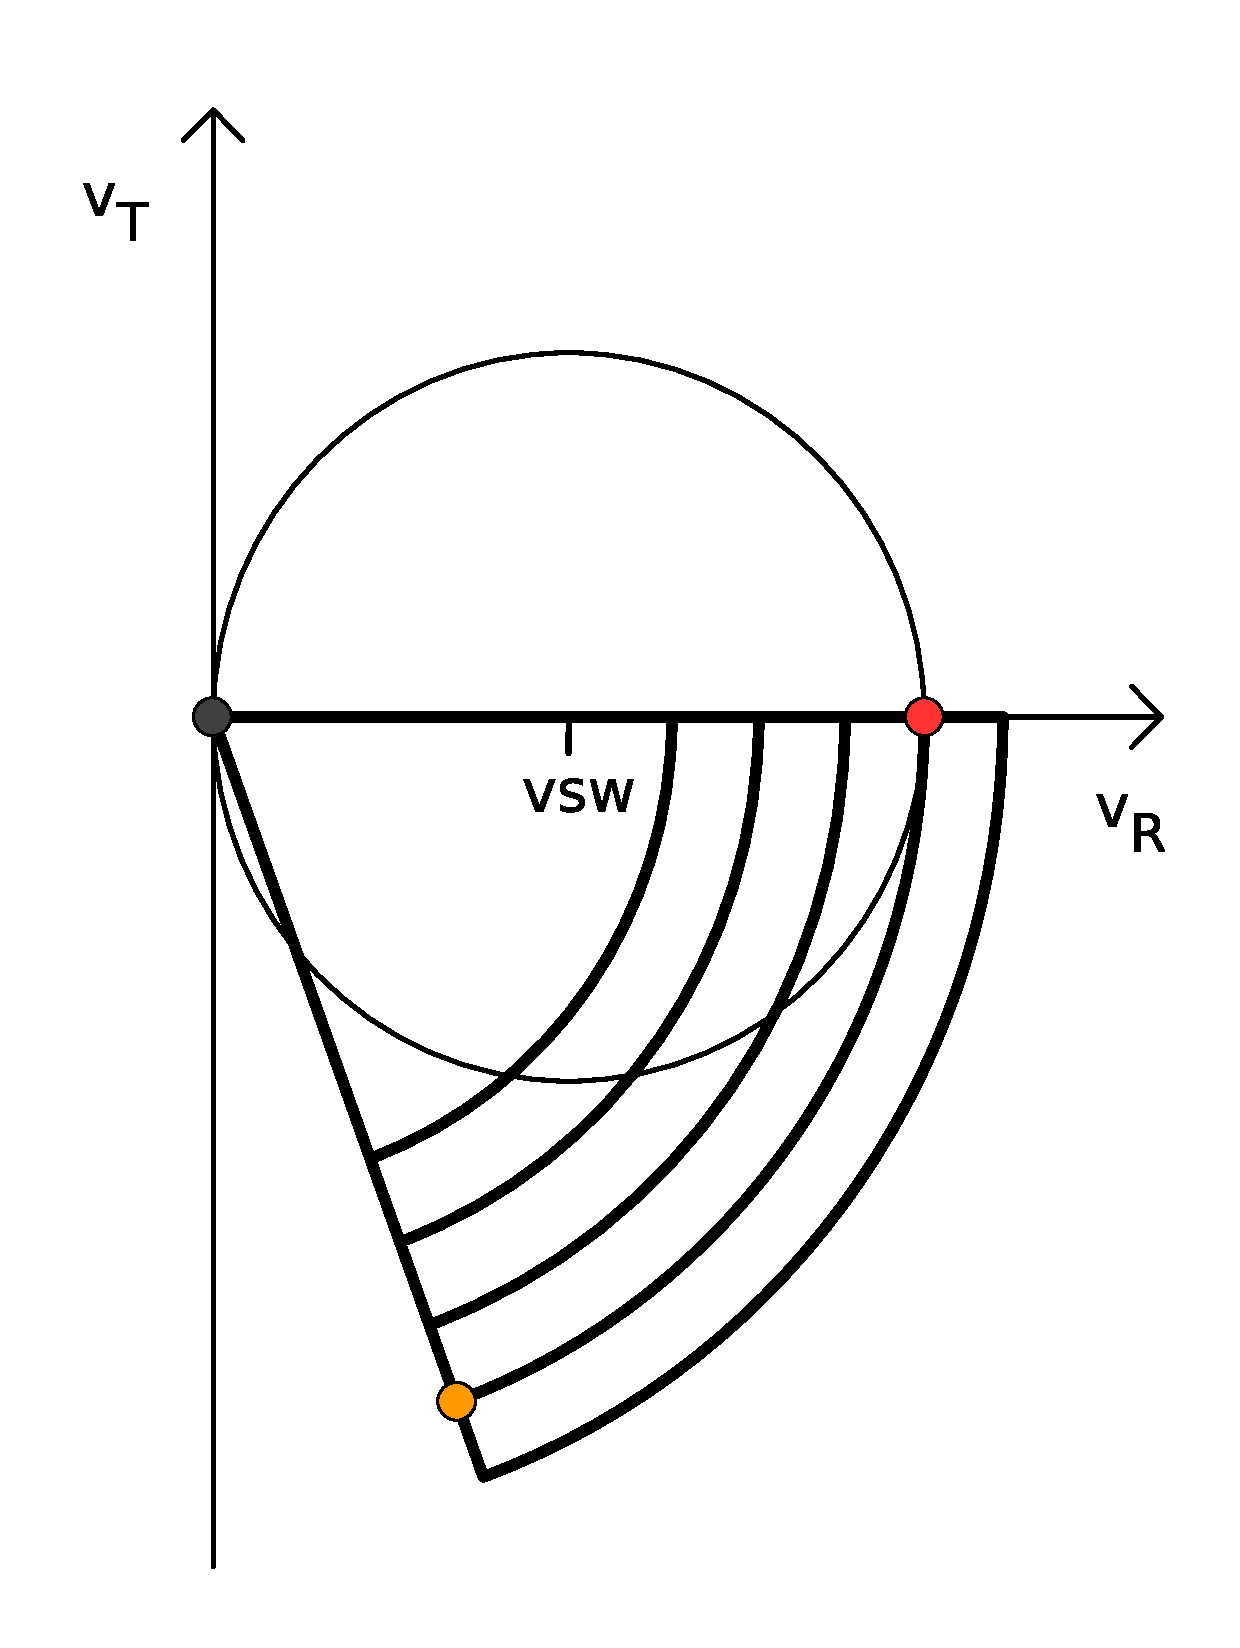
\includegraphics[scale=0.2]{Pics/swics_collimator111.pdf}
%\end{figure}
%\end{columns}
%
%\begin{figure}
%	\vspace{-.5cm}				
%	\includegraphics[scale=0.18]{Pics/qm.pdf}
%	\caption{\tiny{\begin{center}
%				\textit{Gloeckler, Geiss et al., 1992}\end{center}}}
%	
%\end{figure}
%\vspace{0.5cm}
%
%
%\end{frame}

%
%%%%
%\begin{frame}{}
%\begin{columns}
%	\column{4cm}
%	\vspace{-.1cm}
%	\begin{figure}
%		\includegraphics[scale=0.18]{Pics/qm.pdf}
%		\includegraphics[scale=.75]{Pics/slice_R2.pdf}
%	\end{figure}
%	\column{6.5cm}
%	\begin{figure}
%		\includegraphics[scale=.4]{Pics/cart_50_counts_R.pdf}
%	\end{figure}
%\end{columns}
%\end{frame}

%
%
%
\end{document}